\begin{figure}[H]
\center

\includegraphics[scale=1]{kibana.png}
\label{fig:kibana.png}
\end{figure}
\section{Qu'est ce que Kibana}
Kibana est à la fois un front-end à Elasticsearch mais également un outil de présentation
de données puissant. Kibana permet aussi dans une certaine mesure de faire du monitoring.
(avec de grosses guillemets quand même)

Il est principalement codé en angularJS.

C'est l'outil de visualisation officiel d'Elasticsearch, il est assez ergonomique 
et donc plutôt facile d'utilisation. Sa barre de recherche utilise la syntaxe 
search Lite présenté plus dans le chapitre traitant d'Elasticsearch.
Son utilisation pour réaliser des tableaux, dashboard et autre camemberts est assez
aisé une fois les principes de bases assimilés.

\section{Installation de Kibana}
L'installation de Kibana est relativement simple, il suffit de télécharger l'application
compressé à l'adresse sur le site de \url{https://download.elastic.co/kibana/kibana/kibana-4.0.2-linux-x64.tar.gz}{elastic}.
On décompresse, on lance (\ipath{path/bin/kibana}), et c'est parti !

\subsection{Paramétrage}
Afin de pouvoir se connecter à Elasticsearch il faut tout de même renseigner 
\ipath{path/config/kibana.yml} notamment : \emph{port} (par défaut 5601), \emph{host} (ip d'écoute)
et surtout \emph{elasticsearch\_url}.
Dans des circonstances normales c'est tout ce que vous aurez à paramétrer (hors 
SSL \ldots{}).

Il peut arriver dans de rares cas (lorsque Elasticsearch est saturé ou bien lors 
d'une requête particulièrement gourmande) que kibana se ferme car Elasticsearch met
trop de temps à répondre. Il est dans ces cas là, il est fortement conseillé de 
redémarrer l'instance en question, d'étendre sa \emph{HEAP\_SIZE}, ou bien si possible, 
rajouter de la RAM.

Il est possible de modifier le requestTimeout dans \ipath{path/src/lib/waitForEs.js}
C'est pour l'instant la seule façon de faire, d'après une issue github, la prochaine 
mouture de kibana devrait intégrer ce paramètre dans son fichier de configuration.

\section{Utilisation de Kibana}
Dans cette partie nous allons faire une brève présentation (illustré) de Kibana et
de son fonctionnement.

\begin{figure}[H]
\center
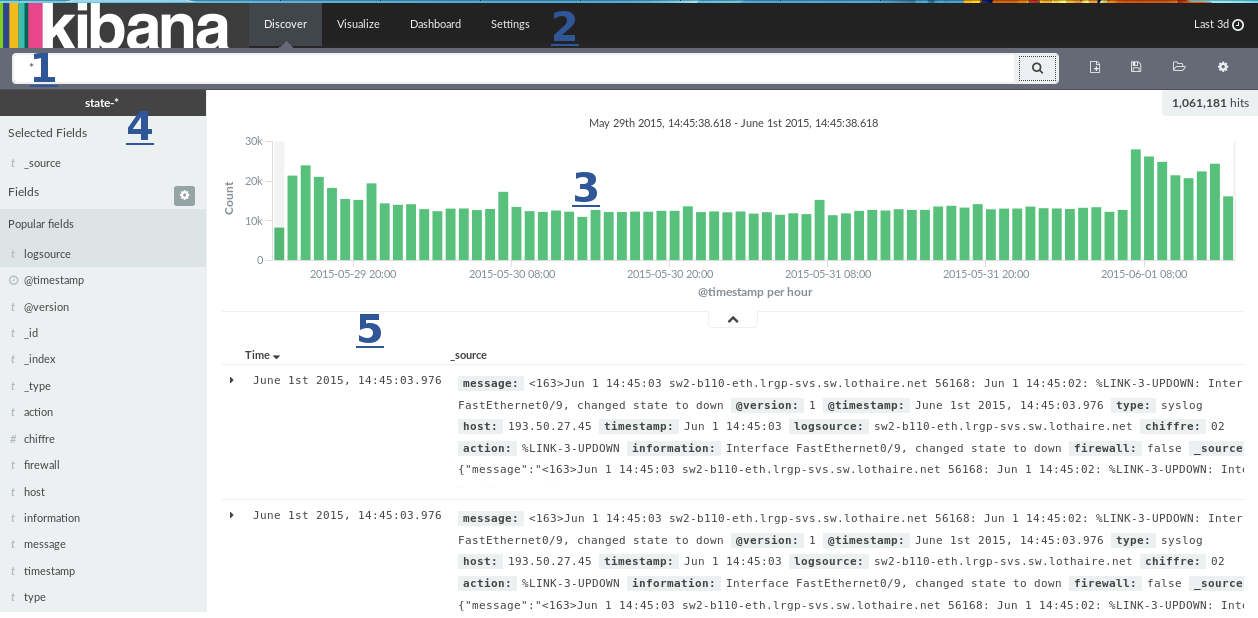
\includegraphics[width=16cm]{kibanatuto/rap/1.png}
\label{fig:kibanatuto1}
\caption{Présentation générale de Kibana}
\end{figure}

Voici la page principale sur laquelle on arrive lorsque l'on se connecte à Kibana
depuis son navigateur.

\begin{enumerate}
    \item La barre de recherche \\(syntaxe SearchLite)
    \item Barre de sélection des \emph{modes} \\(Discover : Recherche, Visualize : Création 
    de Tableaux et autre représentations graphiques, Dashboard : Rassemblement de
    ces présentations, Settings : Paramétrage de certaines options)
    \item Tableau graphique des résultats de recherche
    \item Tableau des champs de l'index
    \item Tableaux des lignes correspondant à la recherche
\end{enumerate}


\begin{figure}[H]
\center
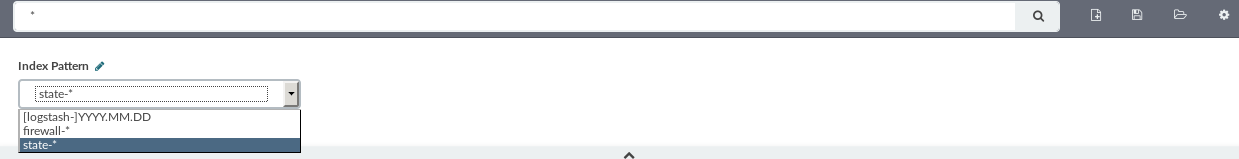
\includegraphics[width=16cm]{kibanatuto/rap/2.png}
\label{fig:kibanatuto2}
\caption{Choisir son index pour une recherche}
\end{figure}
Pour effectuer une recherche, on doit choisir dans quels index, si il est possible 
de réaliser une recherche dans plusieurs index à la fois, il faut dans Kibana que 
ce soit des indexs disposant du même mapping. Typiquement rangés par \ipath{nom-*}.
Pour choisir son index il faut \emph{sélectionner la roue denté à droite de la barre
de recherche}.


\begin{figure}[H]
\center
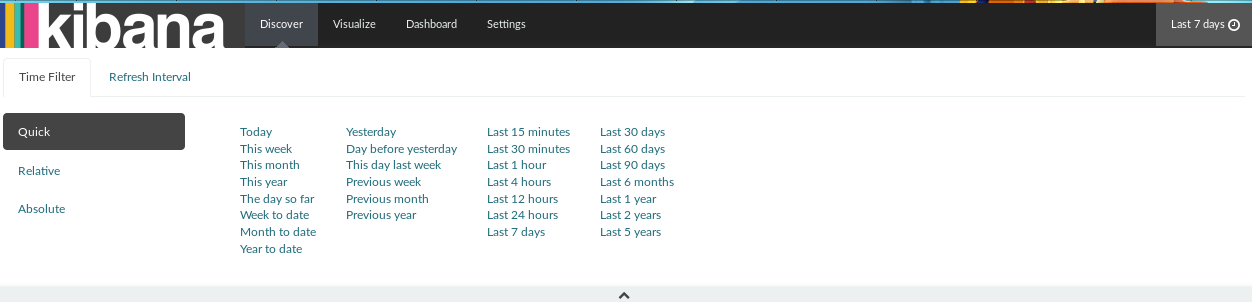
\includegraphics[width=16cm]{kibanatuto/rap/3.png}
\label{fig:kibanatuto3}
\caption{Choisir son intervalle de temps}
\end{figure}
Lorsque l'on effectue une recherche avec Kibana il est possible de choisir de façon
très flexible son intervalle de temps.
Il est tout d'abord possible de de choisir les possibilités du menu rapide, affichées
dans l'image ci-dessus. Le choix est déjà assez exhaustif, mais il est également 
possible de se positionner relativement par rapport à maintenant. Par exemple rechercher 
parmi les 30 dernières secondes, ou bien les deux derniers mois (de la seconde à 
l'année). Il est également possible de choisir un intervalle de temps absolue, à 
la seconde près.

Enfin il est possible de rafraichir ces données en choisissant un intervalle allant
de 5 secondes à une journée (également désactivable).
\newpage
\begin{wrapfigure}{l}{0.3\textwidth}
\begin{figure}[H]
%\center
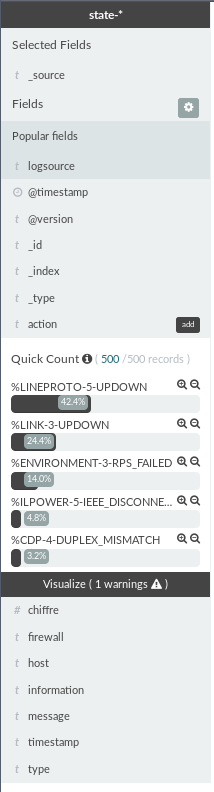
\includegraphics[width=6cm]{kibanatuto/rap/4.png}
\label{fig:kibanatuto4}
\caption{Le tableau des champs}
\end{figure}
\end{wrapfigure}
Le tableau des champs disponibles dans l'index est très pratique pour rendre plus 
lisible les informations que l'on recherche


\section{Ergonomie et dashboards}
